
\chapter{Design and Architecture} % Main chapter title
\label{chap:Chapter5} 
The importance of a correct architecture was already mentioned in the sections \ref{sub:StateOfTheArt_Technology_Architecture} and \ref{sub:architectural_approaches}. For that reason, in this chapter, we will start with an architectural study, where the bet architecture for the system was thought and designed. Although the architecture of a system is a very important step while designing a system, the inner design of the component must not be forgotten. That design will also be presented in this chapter. Furthermore, the domain model of the platform, will also be presented.

%----------------------------------------------------------------------------------------
\section{Architectural Study}
\label{sub:architectural-study} 
In order to have the most correct architecture for the platform in analysis in this dissertation, a study took place, where the system as a whole was examined to see how it would be possible to model an architecture that would fit our system. The name of the platform is SnapTasks.
\par
The first step was to identify how many different front-end applications the system would need. This was done taking into account the existent users groups that exist and their needs. As it was already presented in section \ref{sec:Requirements_userGroups}, there are four main actors: the final customers, the service providers, the courier and, finally, the administrators. The decision of what applications to have was mostly based on the actors that exist, and their needs.
\par

These will be the client applications of the platform: 
\begin{itemize}
  \item \textbf{SnapTasks Website}: the main website of the platform. This is where the users will create their accounts, customers will place their orders and know the available services;
  \item \textbf{\gls{BO} Management}: this application will be responsible for all \gls{BO} and administration operations. Service providers will track their orders in this application;
  \item \textbf{SnapTasks Mobile Application}: similarly to the main website, this will provide essentially the same functions, but on a mobile Android app. Taking into account the graph in figure \ref{fig:mobileGrowth}, it is almost mandatory to have a mobile application, from the beginning;
  \item \textbf{Courier App}: this application allows couriers to check the orders that need pickup and assign themselves to them. This application will also provide the location where the courier needs to pickup/delivery and integrate with the \gls{GPS}.
\end{itemize}

\par
As these applications will be mandatory in our application, one possible architecture would be to keep things to a minimum and have only one \gls{API} that would be responsible to provide all the necessary functionalities to the client apps. Furthermore, it would also be needed a database to persist all the data. Having the minimum number of components means that, in short-term, there will be less development work, the monitoring will also be easier \parencite{monolithProsAndCons}. This architecture is presented in figure \ref{fig:monolithProposal}. 
\par

\begin{figure}[ht]
\centering
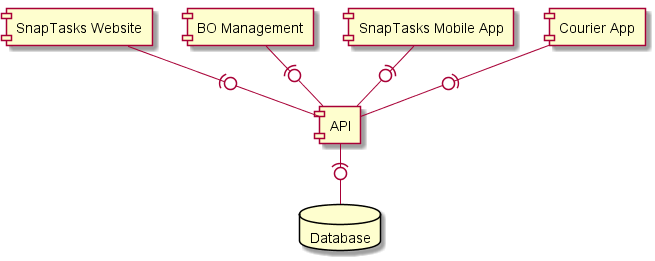
\includegraphics[width=\textwidth,keepaspectratio]{chapters/Architectural_Overview/assets/Monolith.png}
\caption[Possible architectural solution (Monolith)]{Possible architectural solution (Monolith)}
\label{fig:monolithProposal}
\end{figure}

\par

These architectures are known as monolith. This is because all the logic of the system is centred in a single component, without any rule. Monolithic architectures bring more evil than good. With every logic located in the same place, the code can easily become tightly coupled and become very hard to read \parencite{monolithAreBadDesign}. On a logical thinking, it doesn't make sense to provide functions that a certain application will never need. 
\par
In the proposal presented in the figure \ref{fig:monolithProposal}, this happens with the \gls{FO} and \gls{BO} applications. Since each application type needs very different kinds of functionalities. The first ones will need more customer focused operations such as get the available services and placing an order. The second ones need more operational functionalities, like managing service providers or add more services to the platform. 
\par
For that reason, it was decided to split the \gls{API} into two different ones. The first for front-office operations and the second for back-office operations. In this solution, it is possible to segregate the functionalities and restrict its access to the applications that actually, need them. The figure \ref{fig:foBoSeparation} presents an illustration of the possible separation of these functionalities.

\begin{figure}[!hb]
\centering
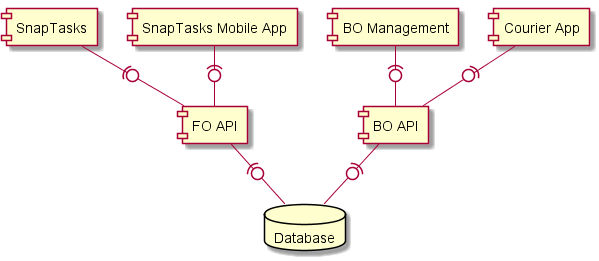
\includegraphics[width=0.9\textwidth,keepaspectratio]{chapters/Architectural_Overview/assets/BoFoSepartion.png}
\caption[Separation of FO and BO APIs]{Separation of FO and BO APIs}
\label{fig:foBoSeparation}
\end{figure}

\par
In this architecture, the separation of allowed not only to separate the concerns of each \gls{API}, but also, to have less load on the services. In case of an unexpected increase of orders, it is possible to temporarily boost the resources of just the FO API, instead of having to upgrade the whole system.
\par
On the other hand, as the application is expected to grow both in terms of number of functionalities and in terms of load, it would be better to have the code even more segmented and decoupled. To achieve this, and as was already explained on section \ref{sub:ExistentSolutions_Architecture_Summary}, a micro-services architecture was designed. 
\par
To design this architecture, it was needed to identify which services were needed and what was their responsibility. From that analysis, the following services were identified: 

\begin{itemize}
  \item \textbf{Pricing Service}: this service is responsible for the creation, calculation and get operations of prices. Each new price that is entered will create a new registry on the database, in order to keep track of the prices and provide a link of the prices that were used in the orders;
  \item \textbf{Order Management Service}: this service is responsible for all the operations that concern the orders. This includes the overall management (create, update), transitions between steps and other logic that is inherent to this entity;
  \item \textbf{Service Provider Management Service}: similarly, this service is responsible for the operations that regard both the service providers and their services. Management operations like create, deactivate and update are under the scope of this service;
  \item \textbf{Courier Service}: the last service is relative to the couriers. Following the previous logic, this service is also responsible to manage the couriers and provide operations that regard the couriers.
\end{itemize}

\par
All services will be bellow both FO API and BO API, which means that those APIs can access the services, but the services can't access the APIs. Furthermore, as the services are only responsible to make operations that only affect the entity in question, there should be no reason for a micro-service to access another micro-service. Lastly, each service is provided a database and the service is responsible to manage it. No service can access the database of another service. The figure \ref{fig:microservicesProposal} presents the proposed architecture.
\par

\begin{figure}[ht]
\centering
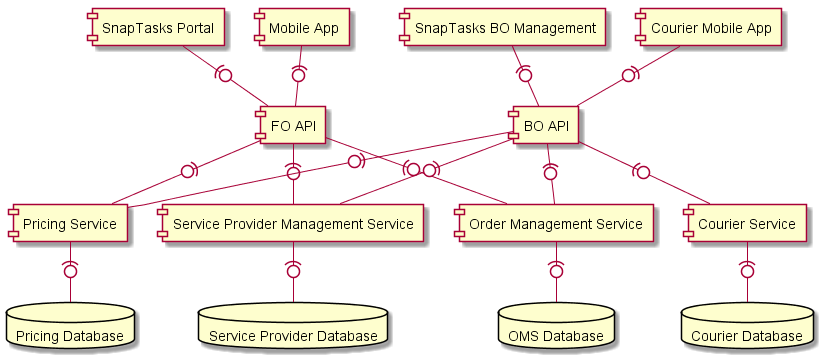
\includegraphics[width=\textwidth,keepaspectratio]{chapters/Architectural_Overview/assets/MicroServices.png}
\caption[Proposal of a Micro-Services Architecture]{Proposal of a Micro-Services Architecture}
\label{fig:microservicesProposal}
\end{figure}


\section{Domain Model}
\label{sec:Implementation_DomainModel}
The design of the domain model is one of the most critical phases in software engineering. This phase not only allows the team to have a better understanding of the business that the application is contained, by helping to identify key concepts and ideas of the business domain, but can also serve as a baseline for the development of a new solution. The domain model is a visual representation of the entities that concern the problem that our application is trying to solve.

\par

With the purpose of having a better understanding of the problem it is being aimed to solve, a domain model was designed. This domain model presents the main concepts and entities that are present in the domain. The figure \ref{fig:domainModel} represents the visual component of the most important concepts on the business domain.



\par
With this visual representation of concepts, it's easier to understand what are the key entities that concern the problem. However, there is still a need to deep dive into these concepts to know what they represent.

\par

The \textbf{order} is one of the most central concepts in the diagram because it is one of the most crucial components of the solution. The whole purpose of the platform is to create and process orders. They are placed by the final \textbf{customer} by interacting with the platform front-end. When the customer places his/her order, it is possible to define where and when he/she desires that the pickup of goods is to be made. This order also has a \textbf{cost}, which is the value that the customer paid for it, which includes both the value for each service, and the logistics fee, for the transportation of goods (including promocodes, if that is the case).
\par
The \textbf{service providers} are another fundamental part of the platform. They are the ones who provide the \textbf{services} that are available on the platform without whom, there would be no orders to be placed. The \gls{SP} also has a \textbf{representative}, which is the point of contact between the provider and the platform. To improve the service quality and avoid orders from customers who are too far away from the \gls{SP}, it is required for the service provider to define an \textbf{area of actuation}. This \gls{AoA} defines a circular area with its center in the \gls{SP}'s address, where it is possible to order from that service provider.
\par
The services that are provided can be of several \textbf{service types} (laundry, mechanics, warranty, etc.), however, for the first version of this application it will only allow laundry services. Nevertheless, the platform is prepared to provide any kind of services. The platform is also prepared to have multiple services gathered in a single order, but as an \gls{MVP}, only one service can be ordered in the front-end.
\par
Each service has its own \textbf{prices}. The price represents the breakdown of what the user will pay por a given service. 
\par

The goods that concern a given order are transported from the customer's and the service provider's \textbf{address} by the \textbf{courier}. This actor is also responsible to assign him/herself to the orders that he/she will deliver. The address contains the necessary information to reach the customer and the service provider, such as name, address info, zip code, city, etc.

\begin{figure}[ht]
\centering
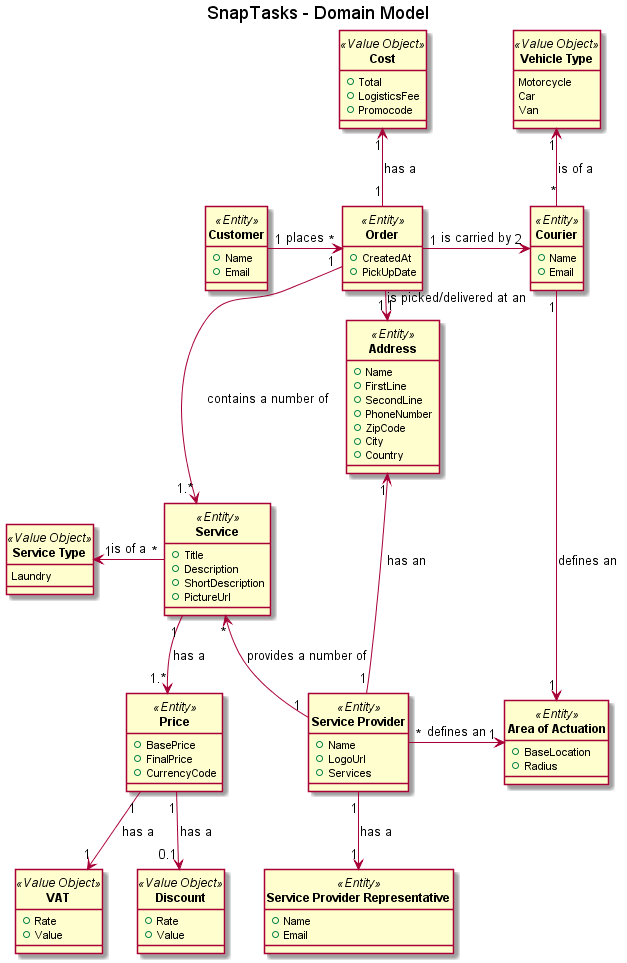
\includegraphics[width=\textwidth,keepaspectratio]{chapters/Architectural_Overview/assets/SnapTasks-DomainModel.png}
\caption[SnapTasks Domain Model]{Snaptasks Domain Model}
\label{fig:domainModel}
\end{figure}

\clearpage
\section{Internal Project Structure}
\label{sec:internal-project-structure}

In the section \ref{sub:architectural-study} the macro architecture of the solution was presented. On the other hand, the internal project structure of each component is still to be presented. The present section is the one where that will be done.

\par

For this solution, each component had an internal layer architecture. This is one of the most common architecture patterns in the industry, and is also known as n-tier architecture pattern. This pattern organizes the application into horizontal layers, each one with its own responsibility, performing a specific role for the application. Despite the nonexistence of a rule for how many layers to exist in a given application, the standard consists in four layers: presentation, business, persistence and database \parencite{softwareArchitecturePatterns}.   

\par

The layered architecture pattern has as one of the most powerful features the separation of concerns among components. The components within a given layer will only need to deal with logic that is that layer's responsibility. For example, the components that are inside the business layer, will only need to deal with business logic. Same applies for the components of the persistence layer, which will only need to have persistence related logic. This makes the components' responsibility easy to define and, by consequence, makes it easier to develop, test and maintain them.

\par

The figure \ref{fig:internalProjectArchitecture} presents the generic layer structure used for the services that compose SnapTasks solution. Despite the layer structure being the same for all components, the biggest difference resides in the \textit{Data} layer. Given that only the bottom services have access to databases, only those services will have a \textit{Repository} and \textit{Database Object \gls{DBO}} sub-layer, since without the need to access a database, there is no need for repository logic and \gls{DBO}. Instead, those services will most likely need to access other services in order to retrieve data. That logic is contained in the \textit{Gateway}.

\par
\begin{figure}[ht]
\centering
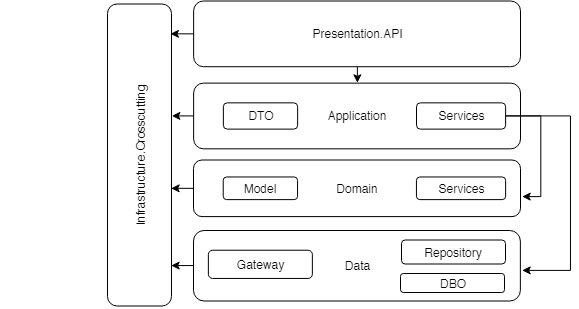
\includegraphics[width=\textwidth,keepaspectratio]{chapters/Implementation/assets/Internal-Service-Architecture.png}
\caption[Generic representation of the internal project structure]{Generic representation of the internal project structure}
\label{fig:internalProjectArchitecture}
\end{figure}

\subsection{Presentation}
\label{sub:InternalStructure_Presentation}
The top layer is named \textbf{Presentation.API} or \textbf{Presentation.Web}, depending if the component is an \gls{API} or an application with \gls{GUI} respectively, is responsible to handle the application's incoming requests. This layer is also responsible to ensure that the incoming data is valid to proceed to the next layer. When the application has a \gls{GUI}, this layer is also responsible to handle the user interaction with the interface. The figure \ref{fig:serviceListingPage}, of section \ref{sub:service-listing-page}, presents the \gls{SLP} of one \gls{SP}.

\par 
In the case of the \glspl{API}, it is possible to check the available endpoints in the \gls{API}'s Swagger page (more information about swagger on section \ref{sub:swagger}).


\subsection{Application}
\label{sub:implementation-application}
The second layer in the chain, \textit{Application}, is the one that is responsible for most of the business logic. This layer is divided into two sub-layers, \textbf{Application.Dto} and \textbf{Application.Services}. The first one is where the \glspl{DTO} are defined. The segregation of this to a separate package, allows to generate a \gls{DLL} that can be used by other projects that need to use this application's \glspl{DTO}. 
\par
The second sub-layer, is the one responsible for the business logic itself. The methods of this layer will be called by the presentation layer, retrieve data from the data layer below, apply the necessary logic and then retrieve it to the presentation layer.

\subsection{Domain}
The \textit{Domain} layer is the one where the domain-related logic is contained. It is divided into two separate sub-layers, \textbf{Domain.Model} where the domain model is specified, and \textbf{Domain.Services}, where domain-related logic (for example, logic that concerns only one object) are implemented. Most of these methods are implemented using as extension methods, and can be used as an extension of the object itself.

\subsection{Data}
The bottom layer is responsible to know where and how to get and persist data in order to the application to work properly. The \textit{Data} layer can be composed by the \textbf{Data.Repository} and \textbf{Data.Dbo}, when the application needs to access a database, and by a \textbf{Data.Gateway}, if it needs to access another application, being that application within the SnapTasks ecosystem, or not. 
\par
The \textit{Data.Dbo} sub-layer is where the \glspl{DBO} are defined. These objects are a representation of the database itself and are needed in order to the used \gls{ORM}, Entity Framework Core, to work properly. These objects are also used by the other sub-layer to access the database. In the \textit{Data.Repository}, all the logic needed to access the database is contained.

\par

In terms of the \textit{Data.Gateway}, it contains all the necessary logic needed to access an external service. As opposed to when we access a repository, we also have ownership of the \glspl{DBO} needed to access, when accessing an external service, that ownership belongs to the application we are calling. The \textit{Data.Gateway} needs to use the \glspl{DTO} provided by that service (also check section \ref{sub:implementation-application}).


\subsection{Infrastructure}

Last, but not least, there is the \textit{Infrastructure} layer. This layer is responsible for the crosscutting concerns that are required by all the other layers. That includes:
\begin{itemize}
    \item Logging
    \item Authorization
    \item Authentication
    \item Mappings
    \item Caching
\end{itemize}
\par

This layer ends up being slightly different from the others because it is not above or below any of the other layers. Instead, it is on the side, and may be accessed by any of the other layers. However, the \textit{Infrastructure} layer can not access any of the remaining layers of the project.